\subsection{FET}
La \textbf{figura~\ref{figura20}} muestra un amplificador en fuente común basado
en JFET es aquel en el que se aplica una señal de entrada de ca a la compuerta y
la señal de salida de ca se toma del drenaje. La terminal fuente es común tanto
para la señal de entrada como para la señal de salida.

\begin{figure}[!ht]
\centering
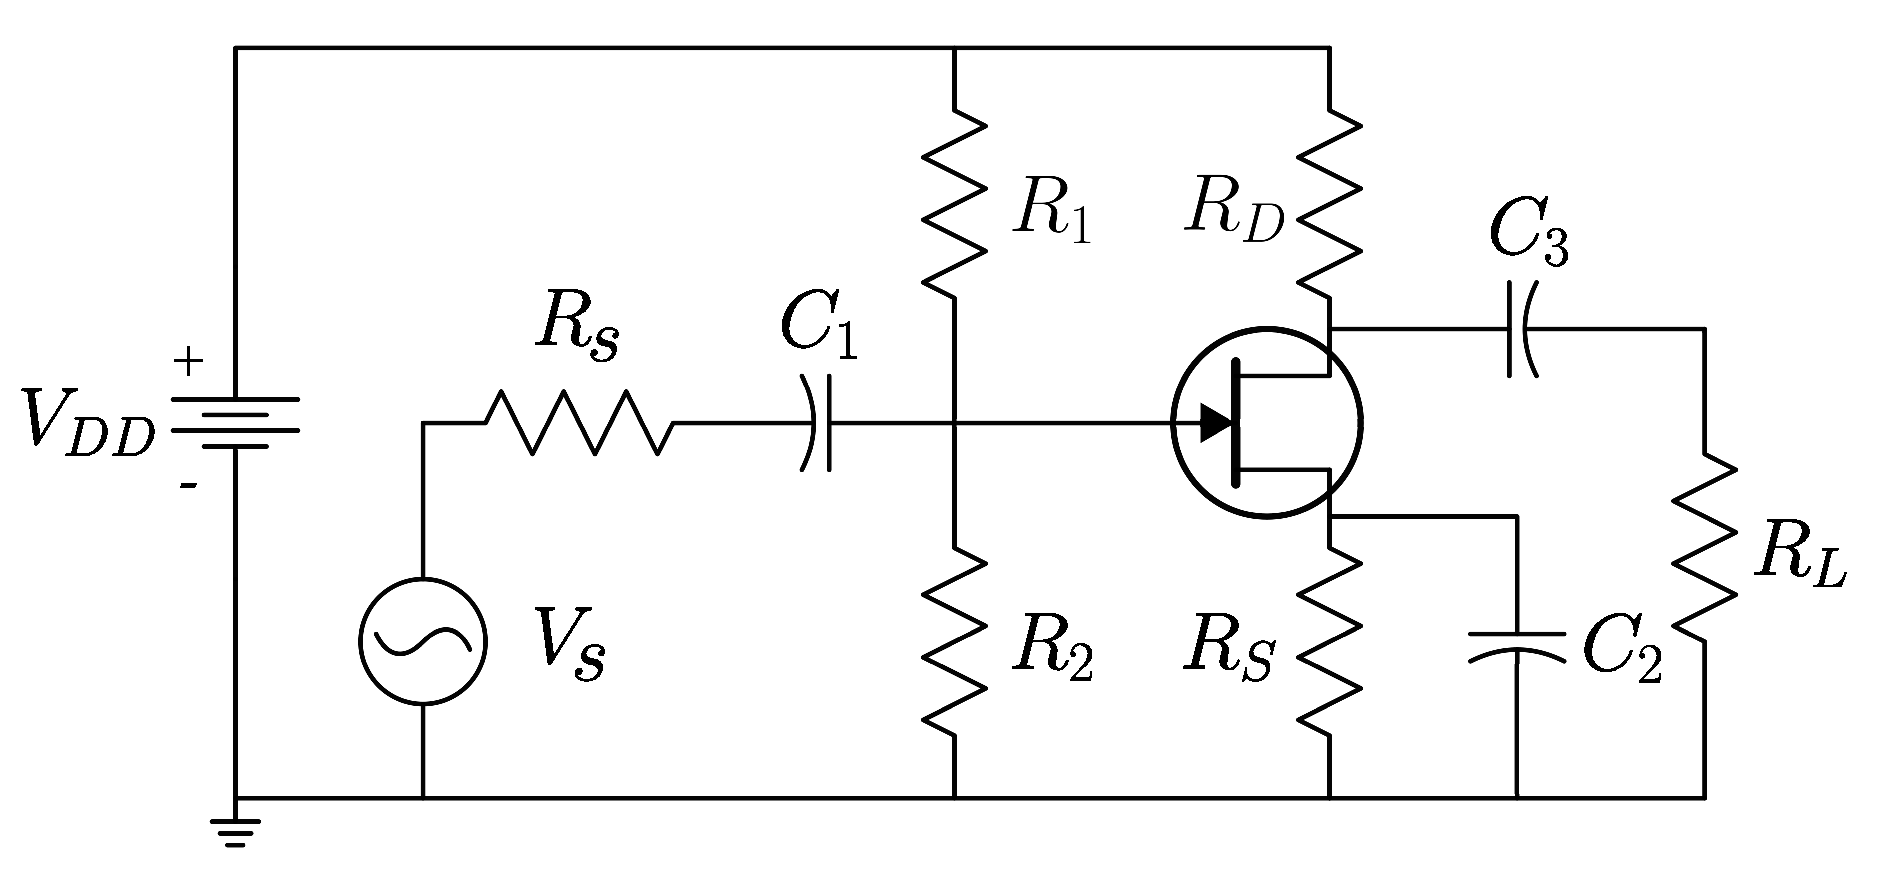
\includegraphics[scale=0.30]{diagramas/figura20.eps}
\caption{Amplificador en fuente común.}
\label{figura20}
\end{figure}

\subsubsection{Calculo de los parámetros del amplificador}
Para hallar los valores del amplificador en fuente común con divisor de voltaje
calculados en la anterior sección se calculan los siguientes valores:

\begin{enumerate}
\item Resistencia interna del generador de funciones:
\begin{equation*}
    R_i = 350[\Omega]
\end{equation*}
\item Transconductancia en $V_{\text{GS}} = 0$:
\begin{equation*}
    g_{\text{m0}} = \frac{2\,I_{\text{DSS}}}{|V_{\text{GS(corte)}}}
                  = \frac{2(\num{15.8e-3}}{|-1.037|}
                  = 0.030473[\text{S}]
\end{equation*}
\item Transconductancia en el punto Q:
\begin{equation*}
    g_{\text{m}} = g_{\text{m0}}\,\left(1 - \frac{V_{\text{GS}}}{V_{\text{GS(corte)}}}\right)
                 = 0.030473\,\left(1 - \frac{-0.209}{-1.037}\right)
                 = 0.024331[\text{S}]
\end{equation*}
\item Resistencia de entrada:
\begin{equation*}
    R_{\text{ent}} = R_1 || R_2
                   = \frac{(1000)(100)}{1000+100}
                   = 90.909[\Omega]
\end{equation*}
\item Resistencia de salida:
\begin{equation*}
    R_{\text{sal}} \cong R_D
                   = 470[\Omega]
\end{equation*}
\item Resistencia de carga:
\begin{equation*}
    R_L = 470[\Omega]
\end{equation*}
\item Ganancia de voltaje:
\begin{equation*}
    A_v = g_m\,\left(\frac{Rd\,Rl}{Rd+Rl}\right)
        = 0.024331\,\left(\frac{(470)(470)}{470+470}\right)
        = 5.7178
\end{equation*}
\end{enumerate}

\subsubsection{Placa de pruebas}
El circuito armado puede verse en la \textbf{figura~\ref{figura21}}, alimentado
por una fuente estable de $9[\text{V}]$ y una señal de corriente alterna
senoidal de $0.1[\text{V}]$ pico a pico.

\begin{figure}[!h]
\centering
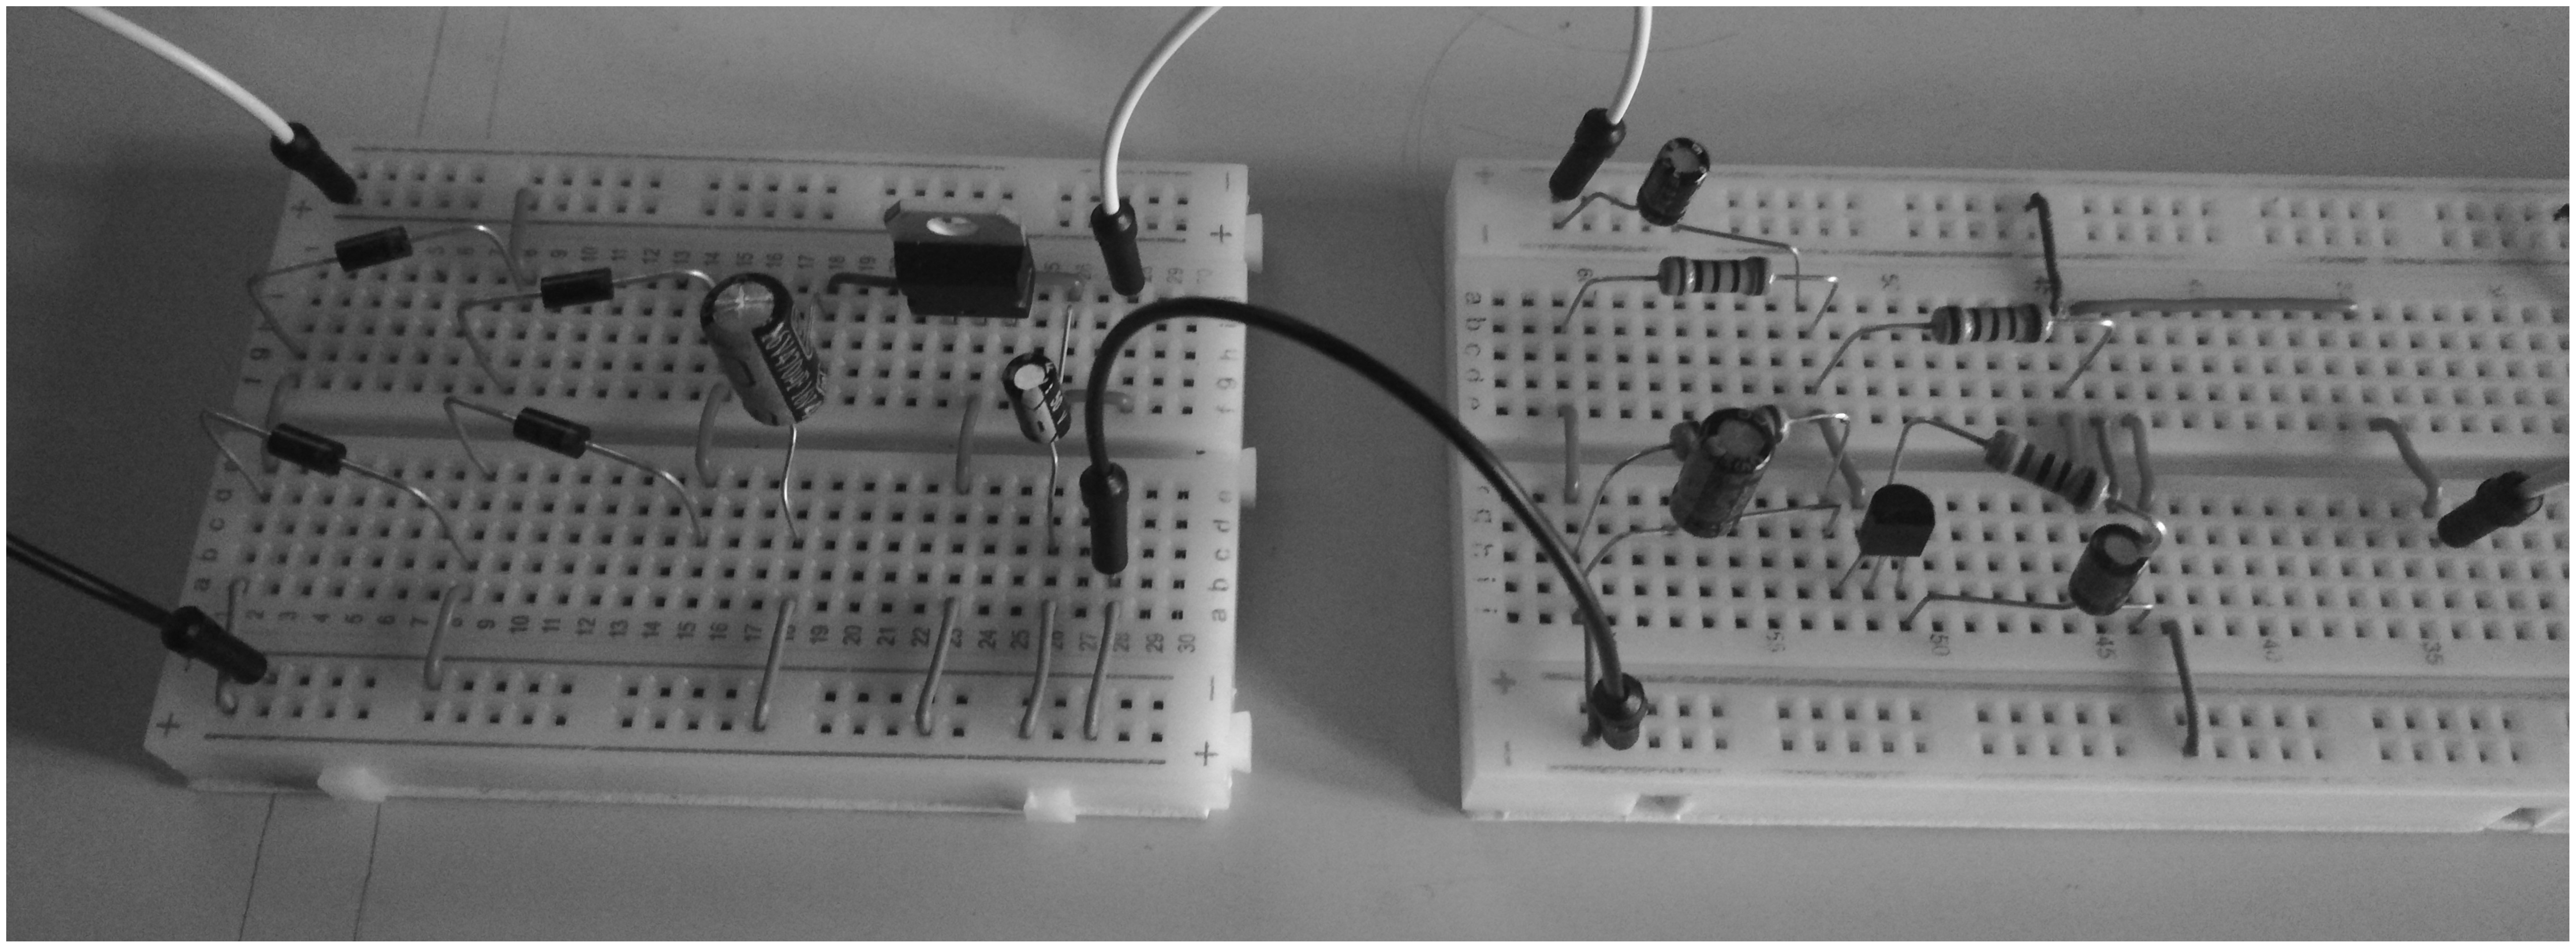
\includegraphics[scale=0.10]{diagramas/figura21.eps}
\caption{Amplificador en placa de pruebas.}
\label{figura21}
\end{figure}

La señal de entrada y la salida del amplificador puede verse en la
\textbf{figura~\ref{figura22}}.

\begin{figure}[!h]
\centering
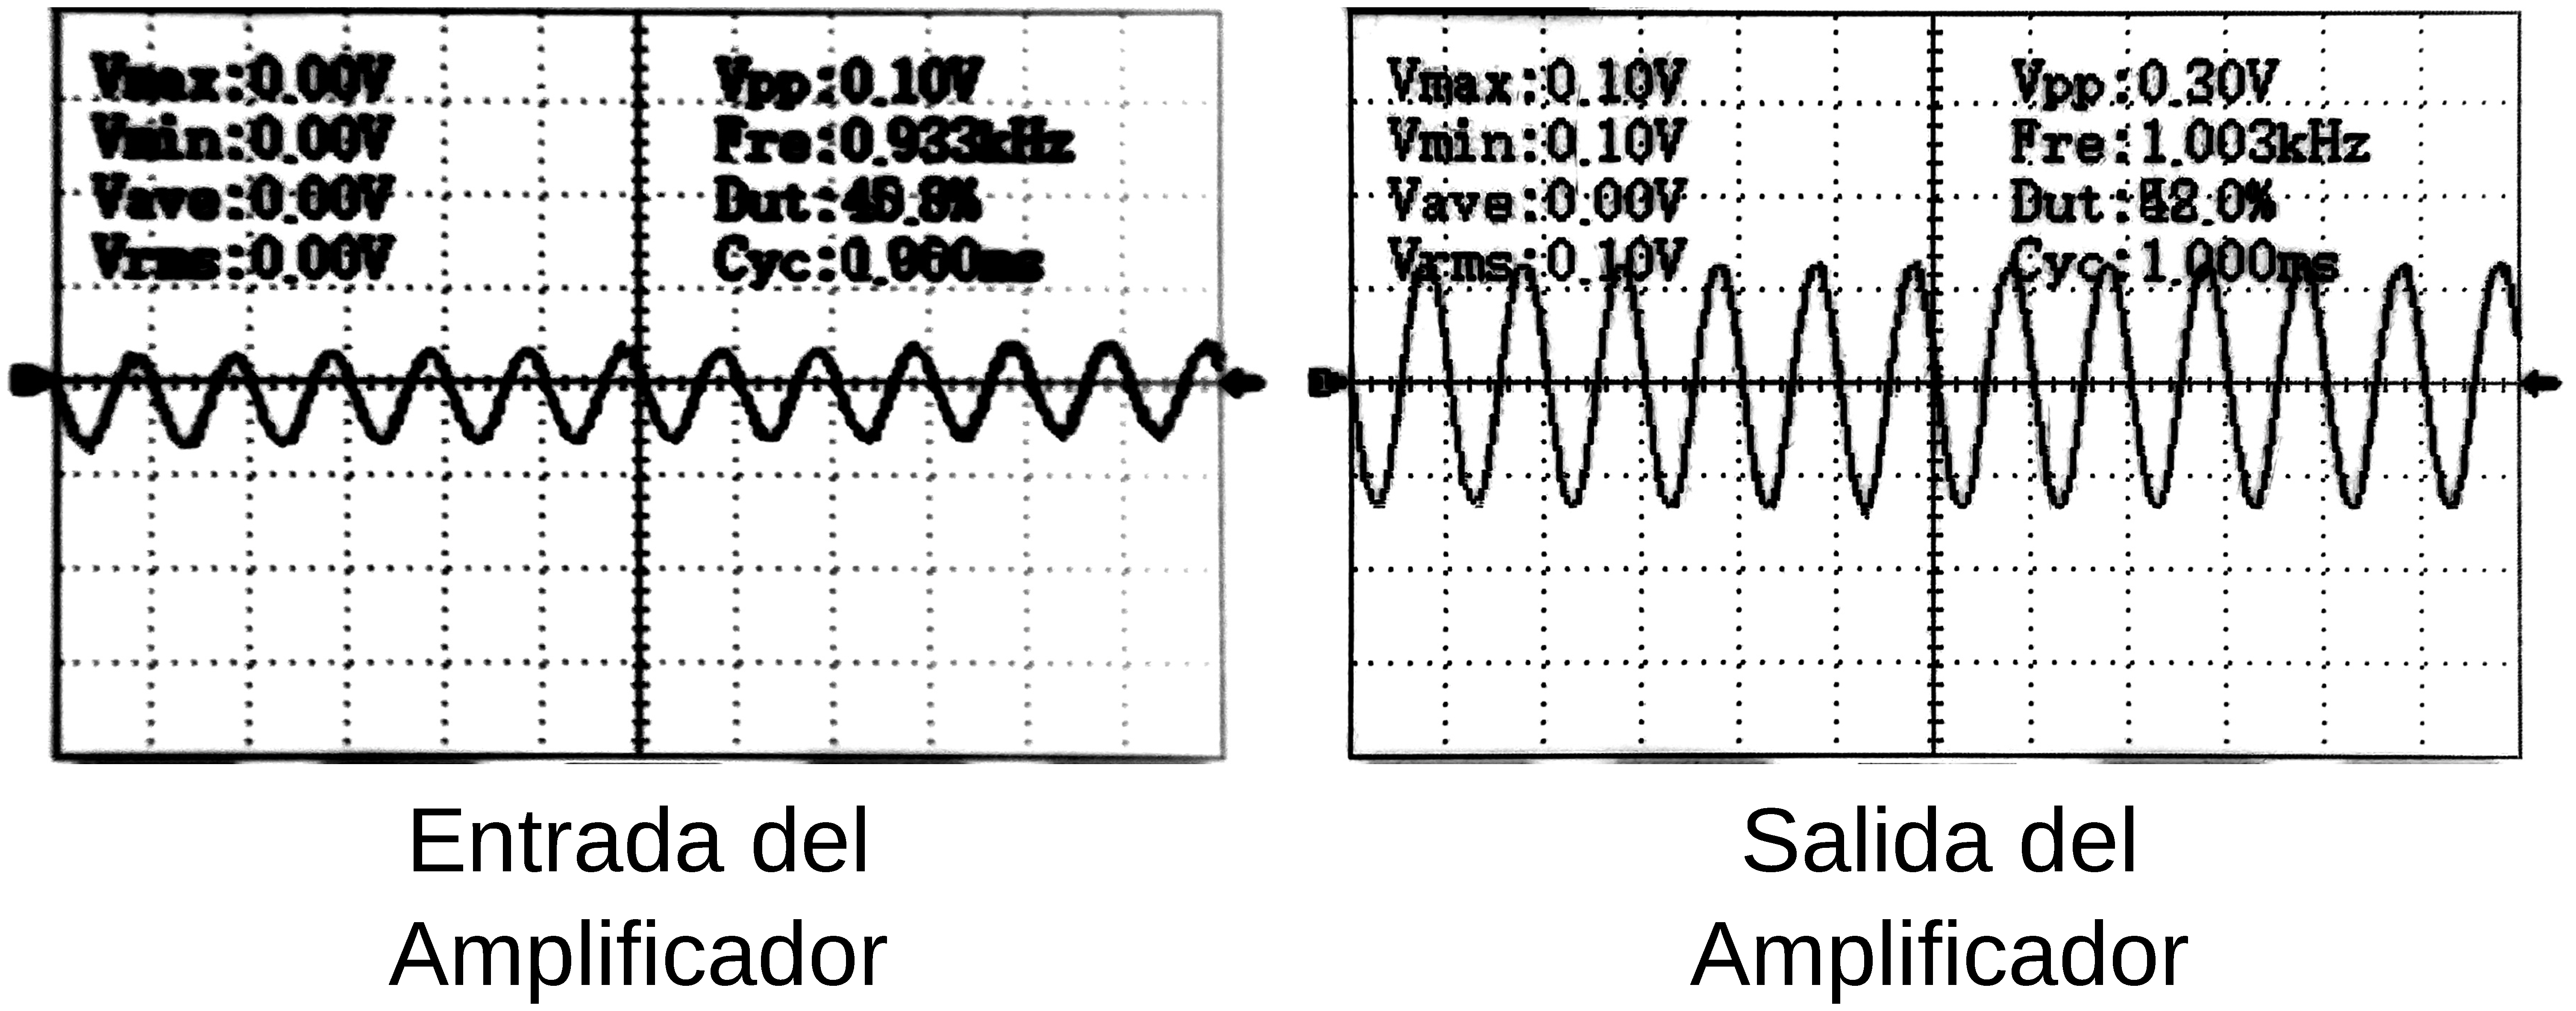
\includegraphics[scale=0.10]{diagramas/figura22.eps}
\caption{Señal de entrada y salida del amplificador.}
\label{figura22}
\end{figure}

